%% LyX 2.4.4 created this file.  For more info, see https://www.lyx.org/.
%% Do not edit unless you really know what you are doing.
\documentclass[english]{article}
\usepackage[T1]{fontenc}
\usepackage[latin9]{inputenc}
\usepackage{units}
\usepackage{enumitem}
\usepackage{amsmath}
\usepackage{amsthm}
\usepackage{geometry}
\geometry{verbose,tmargin=1in,bmargin=1in,lmargin=1in,rmargin=1in}

\makeatletter
%%%%%%%%%%%%%%%%%%%%%%%%%%%%%% Textclass specific LaTeX commands.
\numberwithin{equation}{section}
\numberwithin{figure}{section}
\newlength{\lyxlabelwidth}      % auxiliary length 

%%%%%%%%%%%%%%%%%%%%%%%%%%%%%% User specified LaTeX commands.
\usepackage{fancyhdr}
\usepackage{lastpage}
\pagestyle{fancy}
\usepackage{enumitem}
\usepackage{ifthen}
\everymath=\expandafter{\the\everymath\displaystyle}
%\DeclareMathSizes{10}{10}{10}{10}
\usepackage{multicol}

\usepackage{tikz}
\usetikzlibrary{patterns}
\usetikzlibrary{plotmarks}
\usepackage{pgfplots}
\pgfplotsset{compat=newest}

\usepackage{calc}
\usepackage[nomessages]{fp}

\usepackage{datetime}
% Added by lyx2lyx
\setlength{\parskip}{\smallskipamount}
\setlength{\parindent}{0pt}

\makeatother

\usepackage{babel}
\begin{document}
\renewcommand{\author}{Dr.\,James Ashe}

\newcommand{\classNum}{232}

\newcommand{\classSec}{A and B}

\newcommand{\examType}{Quiz 2 6.2 and 6.3}

\renewcommand{\date}{\formatdate{1}{3}{2013}}

%%First page's header%%%%%%%%%%%%%%%%%%%%%%
\fancypagestyle{firststyle} %%header settings for first pagr
{
	\fancyhead[L]{MTH \classNum{}(\classSec{}) \author{}\\
	\textbf{\examType{}} ~\date{}}
	\fancyhead[C]{\textbf{Name:}}
	\setlength{\headsep}{14pt}
}
%%%%%%%%%%%%%%%%%%%%%%%%%%%%%%%%%%%%%%%%%%

%%Next page's header%%%%%%%%%%%%%%%%%%%%%%%
\setlist{nolistsep}
\lhead{\classNum{}(\classSec{})} 
\chead{\textbf{Name:}} 
\cfoot{\thepage{}~of~\pageref{LastPage}} 
\setlength{\headsep}{5pt} 
%%%%%%%%%%%%%%%%%%%%%%%%%%%%%%%%%%%%%%%%%%%

%%Various settings; see the preamble for other settings%%%%%
%\setenumerate[0]{leftmargin=12pt,itemindent=0pt,labelwidth=0pt}
\setlist{topsep=.5pt}
\renewcommand{\labelenumi}{\textbf{\arabic{enumi}.}}
\renewcommand{\labelenumii}{\textbf{\alph{enumii}.}}
\thispagestyle{firststyle}
%%%%%%%%%%%%%%%%%%%%%%%%%%%%%%%%%%%%%%%%%%

\newcommand{\xmax}{0}
\newcommand{\xmin}{-\xmax}
\newcommand{\xstep}{0}
\newcommand{\ymax}{0}
\newcommand{\ymin}{-\ymax}
\newcommand{\ystep}{0} 

\textbf{Justify your answers and show your work.}

\emph{Find the area of the regions described in the problem.}
\begin{enumerate}[resume]
\item The region bounded by the functions $y=4\sqrt{2x}$, $y=2x$, and
$y=-4x+6$.\\
\noindent\begin{minipage}[t]{1\columnwidth}%

%%%%%%%
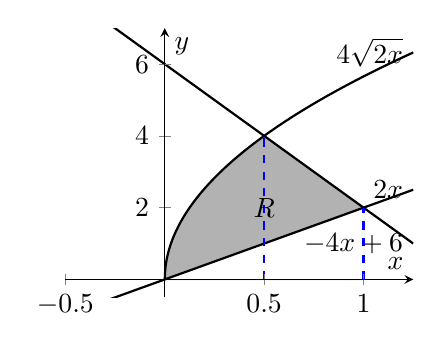
\begin{tikzpicture}
\begin{axis}[height=5cm, 
	width=6cm, 
	axis lines=middle,
	%axis line style={-latex}, 
	xmin=-.5,xmax=1.25, 
	ymin=-.5,ymax=7,
	%restrict y to domain=-1:10,
	%no markers, 
	xlabel={$x$},ylabel={$y$}, 
	%every axis x label/.append style={anchor=north}, 
	%every axis y label/.append style={anchor=east}, 
	area style,tension=0.08]
	
	\addplot+[domain=0:1/2,fill,black!30!white]{4*sqrt(2*x)} \closedcycle;
	\addplot+[domain=1/2:1,fill,black!30!white]{-4*x+6} \closedcycle; 
	\addplot+[domain=0:1,fill,white]{2*x}  \closedcycle;
	
	\addplot[domain=0:1.25,thick,smooth,samples=500]{4*sqrt(2*x)} node[left] {$4\sqrt{2x}$}; 
	\addplot[domain=-1:1.25,thick] {-4*x+6} node[left] {$-4x+6$}; 	
	\addplot[domain=-1:1.25,thick] {2*x} node[left] {$2x$}; 
	
	\addplot[dashed,thick,blue] coordinates{(.5,0) (.5,4)};
	\addplot[dashed,thick,blue] coordinates{(1,0) (1,2)};
	
	\node at (axis cs:.5,2) {$R$};
\end{axis}
\end{tikzpicture}%
\end{minipage}
\end{enumerate}
\vfill

\emph{Let R be the region bounded by the following curves. Use the
disk/washer method to find the volume of the solid generated when
R is revolved about the x-axis.}
\begin{enumerate}[resume]
\item $y=4-x^{2}$, $y=0$, and $x=0$.\\
\noindent\begin{minipage}[t]{1\columnwidth}%

%%%%%%%
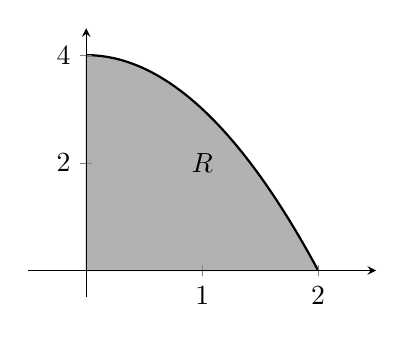
\begin{tikzpicture}
\begin{axis}[height=5cm, 
	width=6cm, 
	axis lines=middle,
	%axis line style={-latex}, 
	xmin=-.5,xmax=2.5, 
	ymin=-.5,ymax=4.5,
	%restrict y to domain=-1:10,
	%no markers, 
	xlabel={$$},ylabel={$$}, 
	%every axis x label/.append style={anchor=north}, 
	%every axis y label/.append style={anchor=east}, 
	area style,tension=0.08]
	
	\addplot+[domain=0:2,fill,black!30!white]{4-x^2} \closedcycle;
	
	\addplot[domain=0:2,thick,smooth,samples=500]{4-x^2}; 
	
	\node at (axis cs:1,2) {$R$};
\end{axis}
\end{tikzpicture}%
\end{minipage}\vfill
\item $y=\sqrt{\sin x}$, $y=1$, and $x=0$.\\
\noindent\begin{minipage}[t]{1\columnwidth}%

%%%%%%%
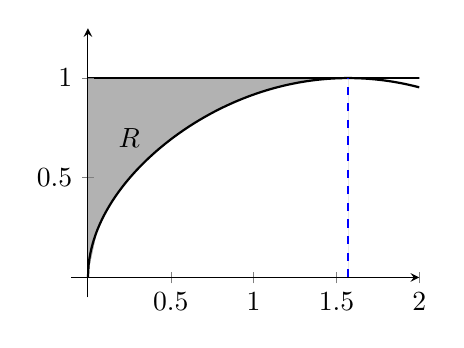
\begin{tikzpicture}
\begin{axis}[height=5cm, 
	width=6cm, 
	axis lines=middle,
	%axis line style={-latex}, 
	xmin=-.1,xmax=2.0, 
	ymin=-.1,ymax=1.25,
	%restrict y to domain=-1:10,
	%no markers, 
	xlabel={$$},ylabel={$$}, 
	%every axis x label/.append style={anchor=north}, 
	%every axis y label/.append style={anchor=east}, 
	area style,tension=0.08]
	\addplot+[domain=0:pi/2,fill,black!30!white]{1} \closedcycle;
	\addplot+[domain=0:pi/2,fill,white]{sqrt(sin(deg(x)))} \closedcycle;
	
	\addplot[domain=0:2,thick,smooth,samples=500]{1};
	\addplot[domain=0:2,thick,smooth,samples=500]{sqrt(sin(deg(x)))};
	\addplot[dashed,thick,blue] coordinates{(pi/2,0) (pi/2,1)};
	
	\node at (axis cs:.25,.7) {$R$};
\end{axis}
\end{tikzpicture}%
\end{minipage}\vfill\newpage
\end{enumerate}
\emph{Use the general slicing method to find the volume of the following
solids.}
\begin{enumerate}[resume]
\item The pyramid with a square base of $4$ meters on a side and a height
of 2 meters (use calculus).\vfill
\item A circular cylinder of radius of radius $r$ and height of $h$ whose
axis is at an angle of $\nicefrac{\pi}{4}$ to the base.\vfill
\end{enumerate}

\end{document}
